
\chapter{Hateville}

\section{Definizione del problema}
\subsection{Istanza}
\begin{itemize}
    \item $X_n = \{1, \dots, n\}$ insieme di $n$ case
    \item $\forall i \in \{1,\dots,n\}$ alla casa $i$ è associato un valore $d_i > 0$
\end{itemize}

\subsection{Soluzione}
{
    \large 
    $$
        S \subseteq X_n : D(S) = \max_{\substack{A \subseteq X_n : \\ \text{comp}(A) = \text{true}}} \{ D(A) \}
    $$ 
}

dove $\forall A \subseteq X_n$
\begin{itemize}
    \item $
    D(A) = 
    \begin{cases}
        \sum_{i \in A} d_i & \text{se } A \not = \emptyset \\
        \emptyset & \text{se } A = \emptyset
    \end{cases} 
    $

    \item $COMP(A) =
    \begin{cases}
        true & \text{se } A \not = \emptyset \land \forall i \in A (i+1 \not \in A \land i-1 \not \in A) \\
        true & \text{se } A = \emptyset \\
        false & \text{altrimenti}
    \end{cases}
    $
\end{itemize}

Se $COMP(A) = true$ diremo che $A$ contiene solo case mutualmente compatibili

\subsubsection{Esempio}
\begin{center}
    \quad $X_6 = \{1, \dots, 6\} \quad n = 6$
    
    \medskip
    \noindent
    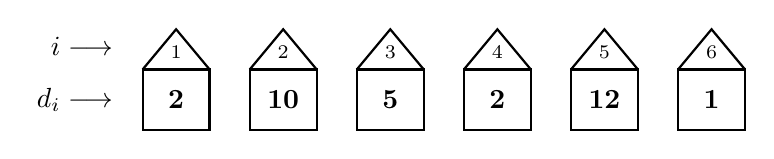
\begin{tikzpicture}[baseline={(0,0.4)}, scale=0.85]
        % Etichette a sinistra con frecce
        \node[anchor=east] at (-0.3, 1.25) {$i \longrightarrow$};
        \node[anchor=east] at (-0.3, 0.45) {$d_i \longrightarrow$};
    
        % Ciclo per disegnare le 6 casette (indice i / valore d_i)
        \foreach \i/\d [count=\x from 0] in {1/2, 2/10, 3/5, 4/2, 5/12, 6/1} {
            \begin{scope}[xshift=\x*1.6cm]
                % Corpo della casa (quadrato)
                \draw[thick] (0,0) rectangle (1,0.9);
                % Tetto (triangolo)
                \draw[thick] (0,0.9) -- (0.5,1.5) -- (1,0.9);
                % Testo: indice nel tetto e valore nel corpo
                \node at (0.5, 1.15) {$\scriptstyle \i$};
                \node at (0.5, 0.45) {$\mathbf{\d}$};
            \end{scope}
        }
    \end{tikzpicture}
    
    \begin{itemize}
        \item $A = \{1, 3, 6\} \qquad \text{comp}(A) = \text{true} \qquad D(A) = 2 + 5 + 1 = 8$
        \item $A = \{2, 5\} \phantom{, 6} \qquad \text{comp}(A) = \text{true} \qquad D(A) = 10 + 12 = 22$
        \item $A = \{2, 3, 5\} \qquad \text{comp}(A) = \text{false}$
    \end{itemize}
    
    \textbf{SOLUZIONE:} \quad $S = \{2, 5\} \quad D(S) = 22$
\end{center}

\newpage
\section{Definizione del sottoproblema}
\subsection{Istanza}
{
    \large

    $$
        \forall i \in \{0,\dots,n\} \quad X_i = \{1,\dots,i\} \quad (X_0 = \emptyset)
    $$
}

\subsection{Soluzione}
{
    \large
    $$
        S \subseteq X_n : D(S) = \max_{\substack{A \subseteq X_n : \\ \text{comp}(A) = \text{true}}} \{ D(A) \}
    $$
}

\subsection{$\mathbf{c_i}$ valore di una massima donazione}
{
    \large
    $$
        c_i = D(S_i)
    $$
}
È il valore di una massima donazione di un sottoinsieme di case mutualmente compatibili

\section{Formulazione ricorsiva}
\subsection{Caso base}
{
    \large
    \begin{itemize}
        \item $\mathbf{i = 0} \quad X_0 = \emptyset \implies S_0 = \emptyset \text{ e }c_0=D(S_0)=0$
        \item $\mathbf{i=1} \quad X_1 = \{1\} \implies \text{ e } c_1=D(S_1) = d_1$
    \end{itemize}
}

Quando $i=1$ $S_i$ e $c_i$ non si possono ricavare dall'equazione di ricorrenza del passo ricorsivo.

Pertanto il caso base contiene 2 sottoproblemi $(i=0 \text{ e } i=1)$ ed è quindi descritto da 2 clausole

\subsection{Passo ricorsivo $\mathbf{i > 1}$}
\begin{itemize}
    \item $\mathbf{i \not \in S_i}$ \\
    $i$ è \uline{inutile} nell'Istanza $X_i = \{1, \dots, \xcancel{i}\}$, quindi risolvere il sottoproblema $i$ equivale a risolvere il sottoproblema $i-1$.

    Pertanto $\mathbf{S_i=S_{i-1} \text{ e } c_i = c_{i-1}}$

    \item $\mathbf{i \in S_i}$\\
    $S_i = S_{?} \cup \{i\} \quad c_i = c_{?} + d_i$\\
    Quale sarà il sottoproblema più piccolo di $i?$ $i-2$| Infatti $S_{i-2} \subseteq X_{i-2}$ $S_{i-2}$ contiene solo case mutualmente compatibili e ciascuna di esse può coesistere con $i$.

    Quindi $\mathbf{S_i = S_{i-2} \cup \{i\} \text{ e } c_i = c_{i-2} + d_i}$
\end{itemize}

Riassumendo
{
    \large
    $$
        S_i = 
        \begin{cases}
            S_{i-1} & \text{se } c_{i-1} > c_{i-2} + d_i \\
            S_{i-2} \cup \{i\} & \text{se } c_{i-1} \leq c_{i-2} + d_i
        \end{cases}
    $$
    $$
        c_i = 
        \begin{cases}
            c_{i-1} & \text{se } c_{i-1} > c_{i-2} + d_i \\
            c_{i-2} + d_i & \text{se } c_{i-1} \leq c_{i-2} + d_i
        \end{cases}
        =
        \max\{c_{i-1},c_{i-2} + d_i\}
    $$
}

\section{Soluzione al problema su istanza $\mathbf{X_n}$}
\begin{itemize}
    \item In termini di \uline{valore della donazione} è $\mathbf{c_n}$
    \item In termini di \uline{sottoinsieme} è $\mathbf{S_n}$
\end{itemize}

\section{Algoritmo bottom-up}
\subsection{Pseudocodice}
\begin{algorithm}
    \begin{algorithmic}
        \Procedure{HV-DON}{$n$}
            \State $c[0]=0$
            \State $c[1] = d_1$

            \For{$i=2$ to $n$}
                \State $c[i] = \max\{c[i-1], c[i-2]+d_i\}$
            \EndFor
        \EndProcedure
    \end{algorithmic}
\end{algorithm}
\subsection{Spiegazione}

\subsection{Complessità}

\newpage
\section{Ricostruzione mediante stampa di $S_i$}
\begin{algorithm}[H]
\caption{\textsc{Print-HV}$(i, c)$}
\begin{algorithmic}[1]
\If{$i == 0$}
    \State \Return
\ElsIf{$i == 1$}
    \State $\text{print}(1)$
\ElsIf{$c[i-1] > c[i-2] + d_i$}
    \State \Call{Print-HV}{$i-1, c$} \Comment{Stampa $S_{i-1}$}
\Else
    \State \Call{Print-HV}{$i-2, c$} \Comment{Stampa $S_{i-2}$}
    \State $\text{print}(i)$
\EndIf
\end{algorithmic}
\end{algorithm}


\section{Ricorstruzione che ritorna $S_i$}
\begin{algorithm}[H]
\caption{\textsc{Set-HV}$(i, c)$}
\begin{algorithmic}[1]
\If{$i == 0$}
    \State \Return $\emptyset$
\ElsIf{$i == 1$}
    \State \Return $\{1\}$
\ElsIf{$c[i-1] > c[i-2] + d_i$}
    \State \Return \Call{Set-HV}{$i-1, c$}
\Else
    \State \Return \Call{Set-HV}{$i-2, c$} $\cup \{i\}$
\EndIf
\end{algorithmic}
\end{algorithm}
